% ------------------------------------------------------------------------------
% TYPO3 CMS 7.4 - What's New - Chapter "Introduction" (English Version)
%
% @author	Michael Schams <schams.net>
% @license	Creative Commons BY-NC-SA 3.0
% @link		http://typo3.org/download/release-notes/whats-new/
% @language	English
% ------------------------------------------------------------------------------
% LTXE-CHAPTER-UID:		9dc37b9a-9fad14c3-bf7eabfd-82b83622
% LTXE-CHAPTER-NAME:	Introduction
% ------------------------------------------------------------------------------

\section{Inleiding}
\begin{frame}[fragile]
	\frametitle{Inleiding}

	\begin{center}\huge{Inleiding}\end{center}
	\begin{center}\huge{\color{typo3darkgrey}\textbf{De feiten}}\end{center}

\end{frame}

% ------------------------------------------------------------------------------
% LTXE-SLIDE-START
% LTXE-SLIDE-UID:		5bcd8641-467360d0-e19379bd-57c3d119
% LTXE-SLIDE-ORIGIN:	3cc566cf-d7166203-45a36415-7c8e8ebf English
% LTXE-SLIDE-ORIGIN:	5d8622ac-37911548-171bf8ec-5add4ed5 German
% LTXE-SLIDE-TITLE:		TYPO3 CMS 7.4 - The Facts
% ------------------------------------------------------------------------------
\begin{frame}[fragile]
	\frametitle{Inleiding}
	\framesubtitle{TYPO3 CMS 7.4 - De feiten}

	\begin{itemize}
		\item Publicatiedatum: 04 augustus 2015
		\item Publicatietype: "Sprint Release"
		\item Visie: Omarm, Innoveer, Verspreid
		\item Primaire focus: Backend makeover Deel 2
	\end{itemize}

\end{frame}

% ------------------------------------------------------------------------------
% LTXE-SLIDE-START
% LTXE-SLIDE-UID:		4d000c5a-269f797e-6f0b6f87-1812802e
% LTXE-SLIDE-ORIGIN:	6746e3bc-a8575d0c-e1681766-d0d78911 English
% LTXE-SLIDE-ORIGIN:	9da27f39-55d99c31-9ee9136a-20d96c0e German
% LTXE-SLIDE-TITLE:		System Requirements
% ------------------------------------------------------------------------------
\begin{frame}[fragile]
	\frametitle{Inleiding}
	\framesubtitle{Systeemvereisten}

	\begin{itemize}
		\item PHP*:\tabto{2.2cm}v5.5.0 - v5.6.x
		\item MySQL:\tabto{2.2cm}v5.5.x - v5.6.x (geen strict mode)
		\item Schijfruimte:\tabto{2.2cm}min 200 MB
		\item PHP instellingen:

			\begin{itemize}
				\item memory\_limit >= 128M
				\item max\_execution\_time >= 240s
				\item compilatieoptie \texttt{--disable-ipv6} \underline{niet} gebruiken
			\end{itemize}

		\item Backend vereist IE >= 9 of een andere moderne browser

	\end{itemize}

	\vspace{1cm}
	*) Meer details: \href{http://typo3.org/news/article/php-minimum-requirements-for-typo3-cms-7/}{PHP Minimum Requirements for TYPO3 CMS 7}

\end{frame}

% ------------------------------------------------------------------------------
% LTXE-SLIDE-START
% LTXE-SLIDE-UID:		06a626bb-9dab63fe-4700886f-634daca7
% LTXE-SLIDE-ORIGIN:	081f8b1d-b8f58841-dccf8d1d-148fd25d English
% LTXE-SLIDE-ORIGIN:	dbbfebbe-fb43ddb8-bca9ae69-716b8a0f German
% LTXE-SLIDE-TITLE:		Development And Release Timeline
% ------------------------------------------------------------------------------
\begin{frame}[fragile]
	\frametitle{Inleiding}
	\framesubtitle{Ontwikkelings- en publicatietijdlijn}

	\begin{figure}
		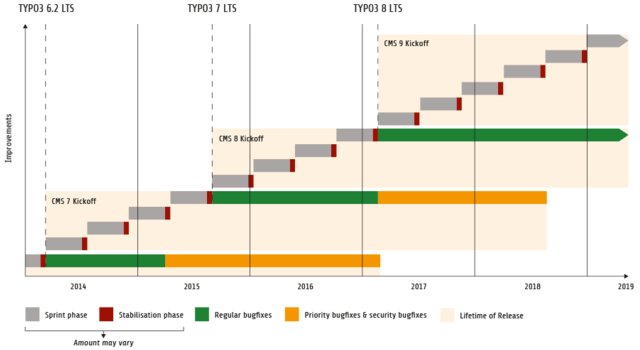
\includegraphics[width=0.90\linewidth]{Introduction/ReleaseAgenda.png}
	\end{figure}

\end{frame}

% ------------------------------------------------------------------------------
% LTXE-SLIDE-START
% LTXE-SLIDE-UID:		aa47832b-b44f337e-cc5b059a-e37b02d4
% LTXE-SLIDE-ORIGIN:	a5555bb0-f1f8031f-f271766a-2dbc1b08 English
% LTXE-SLIDE-ORIGIN:	e359142e-e7c10774-5d851da9-b26a275b German
% LTXE-SLIDE-TITLE:		TYPO3 CMS Roadmap
% ------------------------------------------------------------------------------
\begin{frame}[fragile]
	\frametitle{Inleiding}
	\framesubtitle{TYPO3 CMS Roadmap}

	Geschatte publicatiedatum en primaire focus:

	\begin{itemize}
		\item v7.0 \tabto{1.0cm}02/dec/2014\tabto{3.4cm}Backend makeover deel 1
		\item v7.1 \tabto{1.0cm}24/feb/2015\tabto{3.4cm}Core opschonen en stroomlijnen
		\item v7.2 \tabto{1.0cm}28/apr/2015\tabto{3.4cm}Frontend
		\item v7.3 \tabto{1.0cm}16/jun/2015\tabto{3.4cm}Package Ecosysteem, Composer\newline
			\tabto{3.4cm}en Extensieafhandeling
		\item
			\begingroup
				\color{typo3orange}
					v7.4 \tabto{1.0cm}04/aug/2015\tabto{3.4cm}Backend makeover deel 2
			\endgroup

		\item v7.5 \tabto{1.0cm}29/sep/2015\tabto{3.4cm}\textit{(nog vast te stellen...)}
		\item v7.6 \tabto{1.0cm}xx/xxx/2015\tabto{3.4cm}\textbf{TYPO3 CMS 7 LTS} (Long Term Release)
	\end{itemize}

	\smaller
		\url{https://typo3.org/typo3-cms/roadmap/}\newline
		\url{http://typo3.org/news/article/embrace-and-innovate-typo3-cms-7/}
	\normalsize

\end{frame}

% ------------------------------------------------------------------------------
% LTXE-SLIDE-START
% LTXE-SLIDE-UID:		9c53c404-c177fe81-37220091-eda46212
% LTXE-SLIDE-ORIGIN:	5ef3ad6d-b72464d3-6a2867a6-298cb382 English
% LTXE-SLIDE-ORIGIN:	c8966352-3e5159b9-f0e3ea35-9d4455ef German
% LTXE-SLIDE-TITLE:		Installation
% ------------------------------------------------------------------------------
\begin{frame}[fragile]
	\frametitle{Inleiding}
	\framesubtitle{Installatie}

	\begin{itemize}
		\item Officiële installatieprocedure op Linux/Mac OS X\newline
			(DocumentRoot bijvoorbeeld \texttt{/var/www/site/htdocs}):
		\begin{lstlisting}
			$ cd /var/www/site
			$ wget --content-disposition get.typo3.org/7.4
			$ tar xzf typo3_src-7.4.0.tar.gz
			$ cd htdocs
			$ ln -s ../typo3_src-7.4.0 typo3_src
			$ ln -s typo3_src/index.php
			$ ln -s typo3_src/typo3
			$ touch FIRST_INSTALL
		\end{lstlisting}

		\item Symbolische koppelingen op Microsoft Windows:

			\begin{itemize}
				\item Gebruik \texttt{junction} met Windows XP/2000
				\item Gebruik \texttt{mlink} met Windows Vista en Windows 7
			\end{itemize}

	\end{itemize}
\end{frame}

% ------------------------------------------------------------------------------
% LTXE-SLIDE-START
% LTXE-SLIDE-UID:		374b6c9a-85778e17-0526cb70-765e0c60
% LTXE-SLIDE-ORIGIN:	12551741-9cb07199-fb3614d0-1a242a5f English
% LTXE-SLIDE-ORIGIN:	af099855-2b970b2b-89ed7d02-7219b2b9 German
% LTXE-SLIDE-TITLE:		Upgrade to TYPO3 CMS 7
% ------------------------------------------------------------------------------
\begin{frame}[fragile]
	\frametitle{Inleiding}
	\framesubtitle{Upgrade naar TYPO3 CMS 7.x}

	\begin{itemize}
		\item Upgrade alleen mogelijk van TYPO3 CMS 6.2 LTS
		\item TYPO3 CMS < 6.2 moet eerst naar TYPO3 CMS 6.2 LTS gezet worden
	\end{itemize}

	\begin{itemize}

		\item Upgrade-instructies:\newline
			\smaller\url{http://wiki.typo3.org/Upgrade#Upgrading_to_7.4}\normalsize
		\item Officiële TYPO3 handleiding "TYPO3 Installation and Upgrading":
			\smaller\url{http://docs.typo3.org/typo3cms/InstallationGuide}\normalsize
		\item Algemene aanpak:
			\begin{itemize}
				\item Controleer minimale systeemvereisten (PHP, MySQL, etc.)
				\item Check \textbf{deprecation\_*.log} in oude TYPO3 installatie
				\item Werk alle extensies bij naar nieuwste versie
				\item Zet nieuwe bronbestanden neer en start Install Tool \textrightarrow Upgrade Wizard
				\item Check startmodule voor backend gebruikers (optioneel)
			\end{itemize}
	\end{itemize}

\end{frame}

% ------------------------------------------------------------------------------
